\begin{center}
	
	\begin{tabular}{rp{16cm}lp{20cm}}%{rl}
		
		% after \\: \hline or \cline{col1-col2} \cline{col3-col4} ...
		
		论文地址:& \href{https://dl.acm.org/doi/pdf/10.1145/3437963.3441747}{https://dl.acm.org/doi/pdf/10.1145/3437963.3441747} \\
		来源:& WSDM, 2021 \\
		作者:& Jinze Wu, et al. \\
		单位:& USTC$_{\times 6}$, Anhui University, iFLYTEK Research \\
		源码:& \href{https://github.com/bigdata-ustc/federated-deep-knowledge-tracing}{FDKT} \\
		
		%  slides:& \href{http://yunshengb.com/wp-content/uploads/2017/03/nips_2018_r2l_workshop_talk.pdf}{{\footnotesize Convolutional Set Matching for Graph Similarity}}\\
		
		关键词:& \textbf{Know;edge Tracing, Federated Learning} \\
		
		写于:& \date{2021-09-24}
		
	\end{tabular}
	
\end{center}

该论文\cite{wu2021federated}使用联邦学习来进行Knowledge Tracing。对于以往的方法,论文指出了三个弊端:
\begin{itemize}
	\item Data scarcity:数据不足,学生的学习行为数据通常分散在各个平台以及在线下完成(如何同时使用多个平台的数据)
	\item Different data quality:数据质量不一,各平台/学校的教学安排是不一样的,学生在不同平台上学习并不能连续。例如,不同平台教授Python的过程是不一样的(如何辨别质量低的数据)
	\item Data incompara bility:数据的不一致性,在不同平台学习的学生,他们的知识状态不具有可比性(如何使学生的知识状态一致/对齐)
\end{itemize}
为了解决以上问题,论文提出了一种基于联邦学习的,以Server-client为结构的Knowledge Tracing模型 --- Federated Deep Knowledge Tracing(FDKT)。Client使用单个平台的数据学习,Server负责汇集和更新Clients的参数。


\paragraph{问题定义}
\par{\textbf{Federated Learning(FL)}} 是一种\textbf{保障数据安全}的机器学习方法,一般会有多个clients和一个server,每个client(相当于一个模型)的原始数据都存储在本地,并且不会交换或转移,clients在server的协调下协作解决机器学习问题。

形式化定义:一共有$S$个独立的学校,对于学校$s$,共有$N_s$名学生,$s$中的学生使用问题集是$Q$。一个学生的学习记录:$r = \{(q_1, g_1), ..., (q_l, g_l)\}$,$q_l$表示问题,$g_l \in \{0, 1\}$表示回答。所有学校的问题都是和$K$个知识点相关的。FDKT为每个学校设置一个DKT模型。

\paragraph{FDKT}
FDKT分为clients和server,FDKT学习的过程是一个迭代的过程,在每一次迭代中,每个client需要完成:1)利用所在学习的数据训练DKT模型;2)评估数据的质量。server需要完成:1)接手clients的信息,包括数据质量和模型参数;2)为每个client更新模型参数。


\begin{figure}[h]
	\centering
	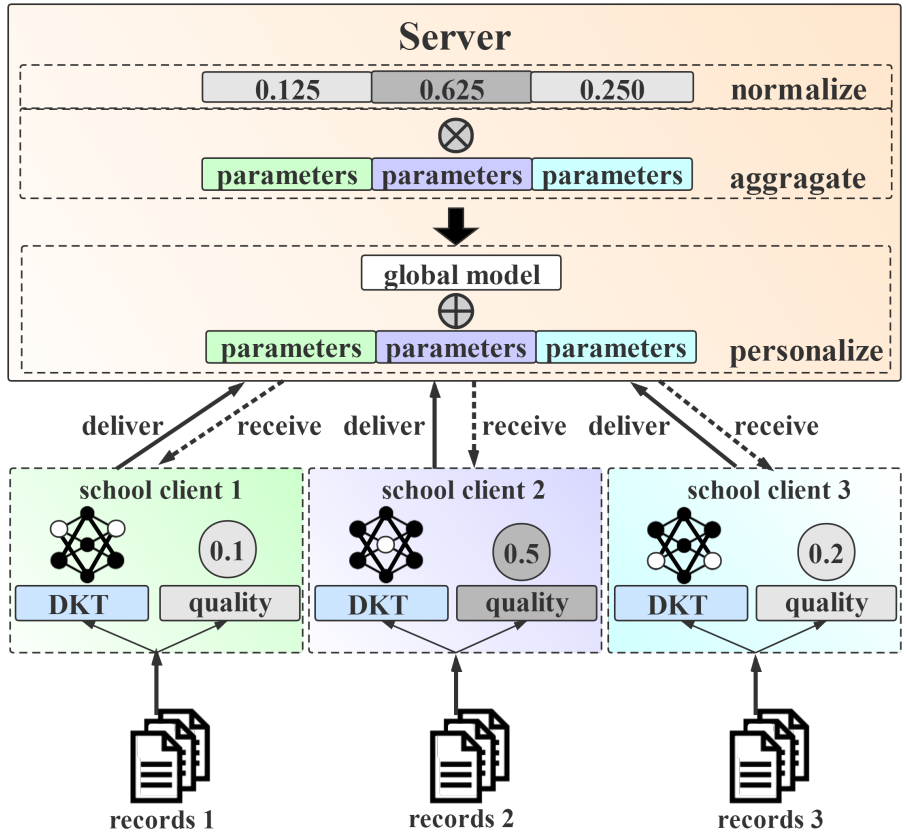
\includegraphics[width=.5\textwidth]{pics/fdkt.png}
	\caption{Federated Deep Knowledge Tracing Framework}
	\label{fig:fdkt}
\end{figure}

FDKT使用的数据集:Math、ASSIST,使用的指标:ACC、AUC、RMSE。

\paragraph{总结}

\begin{itemize}
	\item 考虑了跨平台的数据隐私保护问题
	\item 以联邦学习的方式,融合多个平台的数据,为每个平台训练Knowledge Tracing模型
	
\end{itemize}

